\section{Utilização}

O \textbf{Makefile} é composto apenas por:

\begin{itemize}
  \item \textbf{make}: compila
  \item \textbf{make run}: roda o programa, se conter arquivos temporários, ele o carrega o estado a partir e adiciona todos a \textbf{UnspideredLinks}.
  \item \textbf{make clean}: apaga os arquivos temporários inclusive o dump das \textbf{URLs + HTMLs}.
\end{itemize}

Segue uma imagem do programa em utilização:

\begin{figure}[h]
  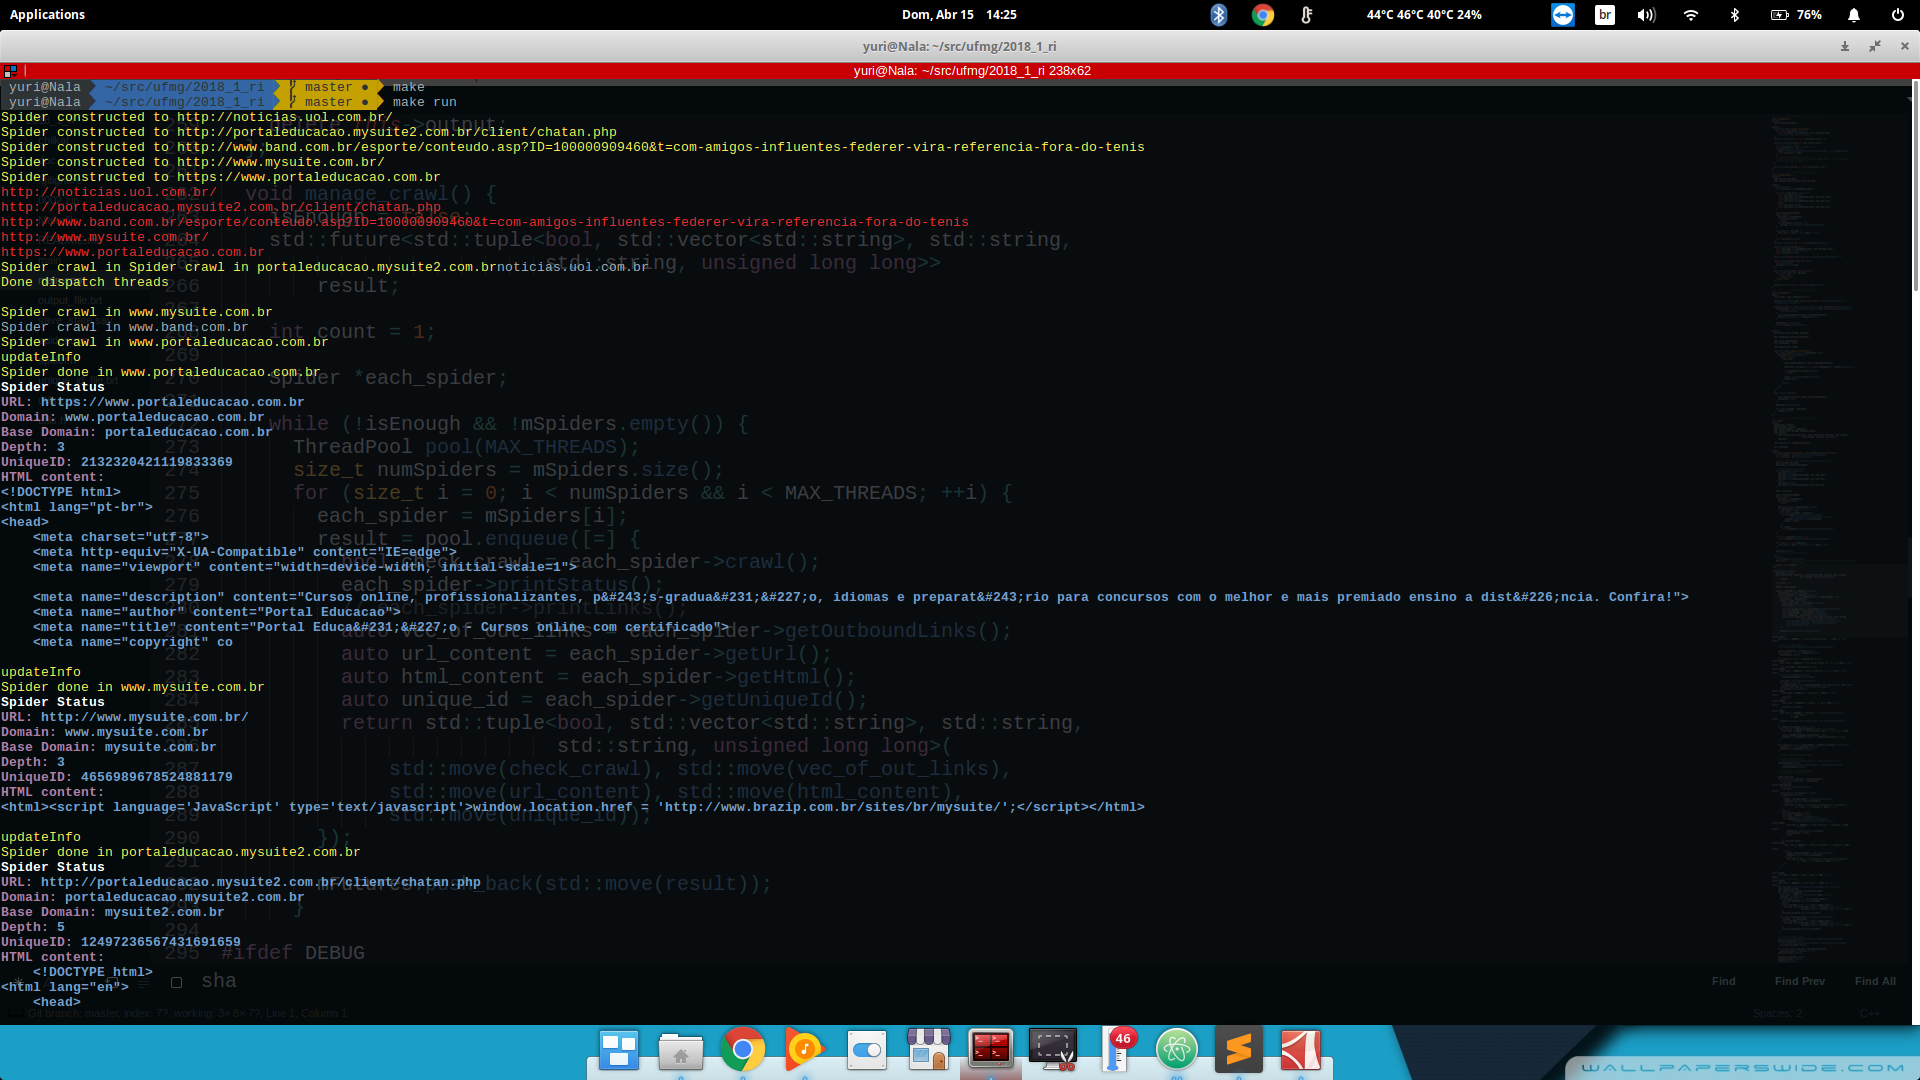
\includegraphics[width=0.5\textwidth]{images/aux2.png}
  \caption{Programa sendo executado}
  \label{fig2}
\end{figure}

Aqui é imprimido a inicialização dos spiders é o que cada spider coletou:

Exemplo:
\begin{itemize}
  \item \textbf{URL}: https://www.portaleducacao.com.br
  \item \textbf{Domain}: www.portaleducacao.com.br
  \item \textbf{Base Domain}: portaleducacao.com.br
  \item \textbf{Depth}: 3

  Profundidade da URL

  \item \textbf{UniqueID}: 2132320421119833369

  ID único para identificar se esta página já foi coletada.

  \item \textbf{HTML content}:

  Conteúdo HTML da página.
\end{itemize}
